\chapter{Estudo de caso: a oscilação ``vai e volta'' do MPC}
\label{cap:caso}

\section{Sintoma}
No Gazebo, com \code{controller\_type: mpc}, o perseguidor oscilava para frente e para
trás ao longo da LOS (período de $\approx$\SI{2,5}{s}). A amplitude crescia até o drone
``se perder''. A análise linear do \cref{cap:discreto} (\cref{tab:margens}) mostrava
margem de fase de \ang{49} com \SI{0,1}{s} de atraso, ou seja, os ganhos \emph{não}
eram o problema.

\section{Reprodução}
Montou-se uma simulação de malha fechada com as bibliotecas C++ reais (MPC + KF), a
malha de velocidade da PX4 (P = 1,8, atitude de 1ª ordem), medida a \SI{30}{Hz} com
\SI{0,1}{s} de atraso e ruído de \SI{0,1}{m}. O alvo anda em reta a \SI{1,5}{m/s}, faz
uma curva entre 15 e \SI{25}{s} e para em \SI{30}{s} (\cref{fig:antes-depois}). O
sintoma apareceu idêntico ao do Gazebo, e o filtro de Kalman foi reiniciado 15--18 vezes
em \SI{40}{s} por rejeição de medidas no \emph{gating}.

\begin{figure}[H]
\centering
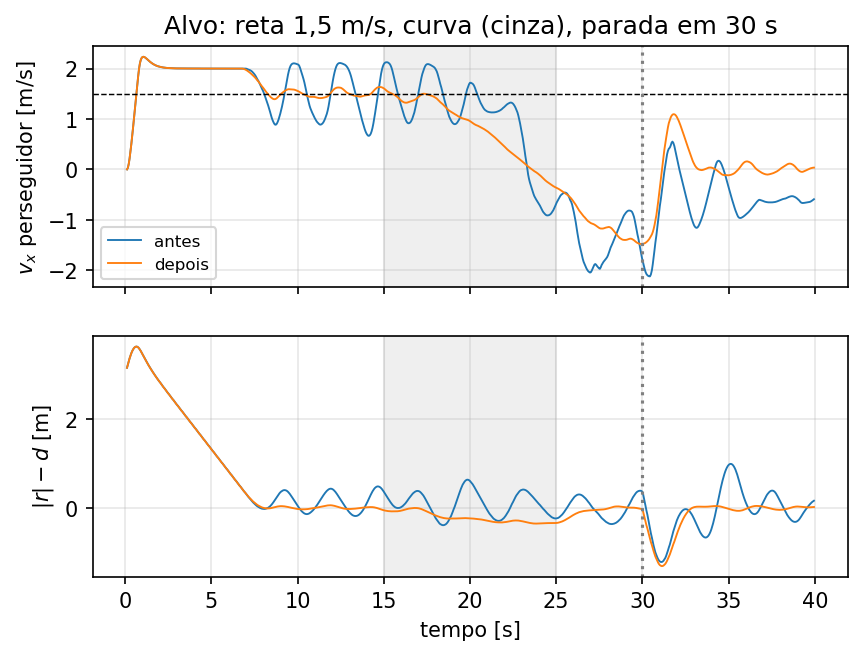
\includegraphics[width=0.85\textwidth]{antes_depois.png}
\caption{Antes e depois das correções (mesmo cenário, mesma semente de ruído).}
\label{fig:antes-depois}
\end{figure}

\section{Causa 1: o KF relativo ignorava a aceleração do perseguidor}
O KF estima $[\rr,\dot\rr]$ \emph{relativos}, num referencial preso ao perseguidor,
supondo $\ddot\rr$ = ruído branco com $\sigma_a=\SI{0,5}{m/s^2}$. Mas
\begin{equation}
  \ddot\rr = \vect a_t - \vect a_c ,
\end{equation}
e o próprio perseguidor acelera até \SI{3}{m/s^2}. Logo:
\begin{enumerate}
  \item a velocidade relativa estimada \textbf{atrasava} em relação à manobra (o filtro
        ``acreditava'' em velocidade constante);
  \item no nó, $\hat{\vect v}_t=\vect v_{c,med}+\hat{\dot\rr}$. Com $\hat{\dot\rr}$ lento,
        $\hat{\vect v}_t$ \textbf{copiava a oscilação do próprio perseguidor} (na simulação,
        0,8--\SI{2,4}{m/s} para um alvo a \SI{1,5}{m/s});
  \item o termo $e_v=v_{ref}-\hat v_t$ do MPC perdia sentido, o amortecimento
        desaparecia e a oscilação crescia;
  \item a inovação do KF crescia até o teste $\chi^2$ rejeitar medidas. Após 5 rejeições
        o filtro reiniciava com $\hat{\dot\rr}=0$, e o drone ``se perdia''.
\end{enumerate}

\paragraph{Correção.} A aceleração do perseguidor é \emph{conhecida} (odometria da PX4).
Ela deve entrar como \textbf{entrada} do modelo, e não como ruído. Com variação linear da
velocidade do perseguidor no intervalo $[t_{k-1},t_k]$,
$\Delta\vect v_c=\vect v_c(t_k)-\vect v_c(t_{k-1})$:
\begin{equation}
  \begin{bmatrix}\rr\\ \dot\rr\end{bmatrix}_k
  = \begin{bmatrix}I & \Delta t\,I\\ 0 & I\end{bmatrix}
    \begin{bmatrix}\rr\\ \dot\rr\end{bmatrix}_{k-1}
  - \begin{bmatrix}\tfrac{\Delta t}{2}I\\ I\end{bmatrix}\Delta\vect v_c + \vect w_k .
\end{equation}
A covariância não muda (a entrada é determinística), e $\sigma_a$ volta a representar só
a aceleração do \emph{alvo}. Implementação: \code{ConstantVelocityKF::predict(dt, frame\_dv)};
o \code{target\_estimator\_node} assina \code{/fmu/out/vehicle\_odometry} e interpola a
velocidade no carimbo de cada medida, como já fazia com a atitude (parâmetro
\code{compensate\_chaser\_motion}). Também se aumentou \code{measurement\_noise\_std} de
0,05 para \SI{0,1}{m}: com ruído real de profundidade de 0,1--\SI{0,15}{m}, o valor 0,05
fazia o \emph{gating} rejeitar medidas boas.

\section{Causa 2: órbita sem amortecimento pela LOS prevista}
Com o alvo parado, o perseguidor continuava girando em torno dele a $\approx$\SI{1,2}{m/s}
com erro de distância nulo. A velocidade de referência do MPC era a derivada
\emph{numérica} de $\vect p_{ref,k}$, construída com a trajetória prevista do próprio
perseguidor. Por \eqref{eq:dep}, a derivada do ponto de standoff contém o termo
\begin{equation}
  +\frac{d}{r}\left(\vect I-\rhat\rhat\T\right)\vect v_c ,
\end{equation}
e em $r=d$ a velocidade tangencial do perseguidor se reproduz \emph{inteira} na
referência. A direção tangencial fica com amortecimento nulo (um modo neutro): qualquer
velocidade tangencial persiste.

\paragraph{Correção.} A referência de velocidade passa a considerar só o movimento do
alvo:
\begin{equation}
  \vect v_{ref,k} = \vect v_t - \frac{d}{\max(r_k,d)}\left(\vect I-\hat{\vect l}_k\hat{\vect l}_k\T\right)\vect v_t .
\end{equation}
Com o alvo parado, $\vect v_{ref}=\vect 0$ e a velocidade tangencial é penalizada. O
MPC dinâmico já usava $\vect v_{ref}=\vect v_t$ e não tinha o problema. Um teste
unitário (\nolinkurl{PredictedLosDampsTangentialDriftAroundStationaryTarget}) falha no
código antigo (deriva de \SI{1,04}{m/s}) e passa no novo.

\section{Resultado}
\begin{table}[H]
\centering
\begin{tabular}{@{}lcc@{}}
\toprule
Métrica (simulação, ruído \SI{0,1}{m}, atraso \SI{0,1}{s}) & Antes & Depois \\
\midrule
Desvio-padrão de $v_x$ em reta (8--\SI{15}{s}) & \SI{0,55}{m/s} & \SI{0,07}{m/s} \\
Reinícios do KF em \SI{40}{s} & 15 & 0 \\
Deriva com alvo parado & \SI{1,06}{m/s} & \SI{0,07}{m/s} \\
RMS do erro de distância na curva & \SI{0,55}{m} & \SI{0,21}{m} \\
\bottomrule
\end{tabular}
\end{table}

\begin{dica}
\textbf{Lição para o TCC.} Em perseguição visual, o desempenho do ``controlador'' depende
tanto do \emph{estimador} quanto da lei de controle. Um ajuste de ganhos não teria
resolvido o problema: a margem de fase já era adequada. Por isso o protocolo do
\cref{cap:comparacao} separa os ensaios com \emph{ground truth} dos ensaios com visão.
\end{dica}
